Finite types\footnote{also called \emph{enumeration types}, however, this usually refers to (a priori mutually disjoint) types with finitely many \emph{uniquely named} elements.} are types with a fixed, finite number of elements. Their predetermined number of elements can be exploited using case distinction. Their usefulness is immediately obvious when trying to formalize e.g. finite groups and functions between them, but they are also ubiquitous in e.g. object-oriented programming languages. Naturally, it is sufficient to have for each natural number $n$ one type with $n$ elements, since all finite types with the same number of elements are isomorphic. Therefore we will focus on this approach, since it conveniently introduces names for the members of finite types and spares us the trouble of having to label them.

\paragraph{} \hypertarget{emptytype}{Starting with the empty type $\emptytype$}, we face the question how to formally declare that this type has no elements. Since we can always declare a new constant \expr{null\mmttp\emptytype} we need to make sure that the existence of this constant leads to a contradiction. We can do so by allowing to construct a term of \emph{any type} given an element of $\emptytype$, which (using Curry-Howard or judgments-as-types) corresponds to the principle \emph{ex falso quodlibet}. There are three ways to go about this:
\begin{enumerate}
	\item Declare a new primitive $\finel eA$ that given $e:\emptytype$ and $A:U$ has type $A$,
	\item use function types and axiomatically declare $\finel\cdot A$ to have type $\emptytype\to A$, or
	\item declare $\emptytype$ to be a subtype of any other type.
\end{enumerate}
The obvious advantage of the second approach is that it allows using $\finel\cdot A$ like an actual typed function. The disadvantage is that using this approach requires function types to be present, hence reducing modularity, and the advantage is negligable. 

The third approach has the advantage that it obviates the need for an elimination form $\finel\cdot\cdot$ completely -- a postulated element $e:\emptytype$ already gives us an element of every other type, namely itself.


\paragraph{} \hypertarget{unit}{Given an additional singleton type $\unit$} with a single element \unite, we can use the coproducts implemented in \autoref{sec:lf:lfx:coprod} to construct the remaining finite types. This way, we can use the elimination form for coproducts to pattern match an element of a finite type, obviating the need for a dedicated elimination form. There are two ways to do this:
\begin{enumerate}
  \item We simply define $\numtp0:=\emptytype$, $\numtp 1:=\unit$, $\numtp 2:=\coprod{\numtp 1}{\numtp 1}$, $\numtp 3:=\coprod{\numtp 1}{\numtp 2}$, etc. The rules for coproducts guarantee, that $\numtp2$ has exactly two elements, namely $\numel0:=\injl\unite{\numtp1}$ and $\numel1:=\injr\unite{\numtp1}$. The elements of $\numtp3$ then are $\numel0:=\injl\unite{\numtp2}$, $\numel1:=\injr{(\injl\unite{\numtp1})}{\numtp1}$ and $\numel2:=\injr{(\injr\unite{\numtp1})}{\numtp1}$. Notably the terms $\numel1:\numtp2$ and $\numel1:\numtp3$ are distinct -- $\numtp2$ is not a subtype of $\numtp3$.
  
  \item If we define \emptytype via subtyping, we can alternatively define $\numtp0:=\emptytype$ or $\numtp0:=\coprod\emptytype\emptytype$, $\numtp 1:=\coprod\unit{\numtp0}$, $\numtp2:=\coprod\unit{\numtp1}$, $\numtp3:=\coprod\unit{\numtp2}$, etc. This way we can use the subtyping rules for coproducts to guarantee that $\numtp i<:\numtp j$ for $i<j$:
  \begin{center}
  	\begin{tabular}{rlll}
		$\numel 0$ & $:= \injl\unite\emptytype$ & $:\numtp1:=\coprod{\unit}{\numtp0}$ & $<:\coprod\unit N$ \\
		$\numel 1$ & $:= \injr{(\injl\unite\emptytype)}\unit$ & $:\numtp2:=\coprod\unit{\numtp1}$ & $<:\coprod\unit{(\coprod\unit N)}$ \\
		$\numel 2$ & $:= \injr{(\injr{(\injl\unite\emptytype)}\unit)}\unit$ & $:\numtp3:= \coprod\unit{\numtp2}$ & $<: \coprod\unit{(\coprod\unit{(\coprod\unit N)})}$
	\end{tabular}
	\end{center}
	and $\numel i$ is the same expression at all numerical types. In particular, we can easily define the successor function as $\cn{succ}(n):=\injr n\unit$.
\end{enumerate}
Conveniently, defining \emptytype to be a subtype of any other type allows for implementing both variants.

\paragraph{} In the presence of function types, we can also define \unit as $\lfarrow\emptytype\emptytype$, knowing that the only possible inhabitant of this type is the function $\unite=\lflambda{x:\emptytype}x=\lflambda{x:\emptytype}{\finel x\emptytype}$. However, even using this definition, we still have to provide a rule for the solver to be able to exploit this knowledge (and to make sure that $\finel x\emptytype$ is the identity).

All of this leaves us with several options listed in \autoref{fig:lf:lfx:finite:impls} and the basic rules in \autoref{fig:lf:lfx:finite:rulesbasic}.

\begin{figure}[ht]\centering
\resizebox{\textwidth}{!}{
\begin{tabular}{r||c|c|c|c}\tiny
	& \emptytype & \unit & \textbf{higher finite types} & \textbf{elimination} \\\hline\hline
	\textbf{finite types} & primitive $\finel\cdot\cdot$ & primitive & primitive & dedicated case construct \\\hline
	\textbf{finite types + \coprodsym} & primitive $\finel\cdot\cdot$ & primitive & definable using \coprodsym & \cmatchsym-terms \\\hline
	\textbf{finite types + $\lfpisym$} & $\finel\cdot A : \lfarrow\emptytype A$ & $\begin{aligned}\unit&:=\lfarrow\emptytype\emptytype\\\unite&:=\lflambda{x:\emptytype}x\end{aligned}$ & primitive & dedicated case construct \\\hline
	\textbf{finite types + \coprodsym + $\lfpisym$} & $\finel\cdot A : \lfarrow\emptytype A$ & $\begin{aligned}\unit&:=\lfarrow\emptytype\emptytype\\\unite&:=\lflambda{x:\emptytype}x\end{aligned}$ & definable using \coprodsym & \cmatchsym-terms 
\end{tabular}}
(column $\emptytype$ can be replaced by a subtyping rule)
	\caption{Possible Implementations for Finite Types}\label{fig:lf:lfx:finite:impls}
\end{figure}

\begin{figure}[ht]%[ht]\centering%\vspace*{-1em}
\begin{framed}
{\small For any $U$ with $\gjudg{\judguniv U}$:}
\begin{flushleft}
\textbf{Formation:}
\[
\trule{}{\gjudg{\infertype\emptytype\type}} \qquad \trule{}{\gjudg{\infertype\unit\type}}
\]
\textbf{Introduction:}
\[
\trule{}{\gjudg{\infertype\unite\unit}}
\]
\textbf{Elimination:}
\[
\trule{\gjudg{\hastype e\emptytype} \quad \gjudg{\infertype AU}}{\gjudg{\infertype{\finel eA}A}}
\]
%\textbf{Type Checking:}
%\[
%\_
%\]
\textbf{Equality:}
\[
\trule{}{\gjudg{\judgeq ab\unit}}
\]
\textbf{Computation (Optional):}
\[\ \trule{\gjudg{\infertype AU}}{\gjudg{\judgeqc{\finel eA}e}} \]
\textbf{Subtyping (Optional):}
\[ \trule{\gjudg{\infertype AU}}{\gjudg{\subtp\emptytype A}} \]
%\textbf{Computation (Optional):}
%\[
%	\trule{}{\gjudg{\judgeqc\unit{\emptytype\to\emptytype}}}
%\]
\end{flushleft}\end{framed}%\vspace*{-.5em}
\caption{Basic Rules for Finite Types}\label{fig:lf:lfx:finite:rulesbasic}%\vspace*{-1em}
\end{figure}

\paragraph{} Of course, constructing enumeration types and their elements by nesting \coprodsym-types and injections is simple to formally specify and implement, but inconvenient to use in practice. Furthermore, while it is possible to build up enumeration types using \coprodsym even in the absence of coproducts by adapting their rules, the most general and user-friendly way to implement finite types is via a primitive type constructor on actual integers. 

We can do so using a type \nat of number literals, which we discuss further in \autoref{sec:lf:lfx:literals}: \hypertarget{enum}{We implement a type constructor $\enum i$ for the type $\numtp i$, and analogously a constructor $\enume ij$ for $\numel i:\numtp j$.} In this case, it is desirable that $\enum x$ is a valid type even if $x$ is a variable or otherwise undetermined and $\enume xj$ checks against type $\enum j$ iff $x<j$. If $x$ and $j$ are not definite number literals, this implies proving a judgment $\gjudg{x<j}$, which requires corresponding proof rules for the ordering on natural numbers and a way for the user (and the solver) to construct (and find) such proofs.

If we want to consider enumeration types as subtypes of each other, the argument $j$ in $\enume ij$ becomes unnecessary, so we can write $\enumu i$ instead.

\begin{remark}
	In service of clarity, I will not introduce object-level judgments here, since they require corresponding proof rules which are not really relevant for this chapter. Suffice it to say that \mmt offers a method *Solver.prove(tm : Term)*, that returns *true* if and only if the Solver manages to find \emph{any} element *p* of type *tm*. This method can cover premises of the form $\gjudg{x<y}$ for any choice of object-level judgments (and their proofs). Of course this immediately makes type checking undecidable, and the power of the rule system ultimately depends on the power of the internal prover, which in the case of \mmt is rather weak.
\end{remark}

\autoref{fig:lf:lfx:finite:rulesext} gives a set of rules for these \enumsym-types, where $\numtp n$ represents the (or any variant of, in the case of subtyping) \emph{defined} finite type corresponding to the (definite) number literal $n$, and $\numel n$ represents an element of such a type (again, for a definite number $n$). Which of the optional rules to implement depends on which of the implementation approaches discussed above we choose.
\begin{figure}[ht]%[ht]\centering%\vspace*{-1em}
\begin{framed}
% {\small For any $U$ with $\gjudg{\judguniv U}$:}
\begin{flushleft}
\textbf{Formation:}
\[
\trule{\gjudg{\hastype i\nat}}{\gjudg{\infertype{\enum i}\type}}
\]
\textbf{Introduction:}
\[
\trule{\gjudg{\hastype i\nat}\quad\gjudg{\hastype j\nat}\quad\gjudg{i < j}}{\gjudg{\infertype{\enume ij}{\enum j}}}\qquad
\left( \trule{\gjudg{\hastype i\nat}}{\gjudg{\infertype{\enumu i}{\enum{i+1}}}} \right)
\]
\textbf{Elimination:}
\[
\text{(pattern match rule)}
\]
\textbf{Type Checking (Optional):}
\[
	\trule{\gjudg{i<j}}{\gjudg{\hastype{\enumu i}{\enum j}}}
\]
\textbf{Equality:}
%\[
%\_
%\]
\textbf{Computation (Optional):}
\[ 
	\trule{}{\gjudg{\judgeqc{\enum n}{\textbf n}}} \qquad
	\trule{}{\gjudg{\judgeqc{\enumu n}{\underline n}}} 
\]
\textbf{Subtyping (Optional):}
\[ \trule{\gjudg{i < j}}{\gjudg{\subtp{\enum i}{\enum j}}} \]
%\textbf{Computation (Optional):}
%\[
%	\trule{}{\gjudg{\judgeqc\unit{\emptytype\to\emptytype}}}
%\]
\end{flushleft}\end{framed}%\vspace*{-.5em}
\caption{Convenience Rules for Finite Types}\label{fig:lf:lfx:finite:rulesext}%\vspace*{-1em}
\end{figure}

\paragraph{} To summarize: Finite types give us various ways of implementing their different aspects, depending on which additional typing features are available in any context and how we want them to behave with respect to subtyping. Note however, that implementing all constructors as primitives still allows us to reuse the \emph{symbols} already implemented for other typing features: A primitive elimination form for finite types can reuse the \cmatchsym-symbol from the \expr{Symbols} theory for coproducts, and we can reuse the \coprodsym-symbol to construct higher finite types even in the absence of the rules governing coproducts. Even the rules governing these symbols can be reused with minimal adaptation (to restrict the types that are valid arguments to finite types).

This allows for developing library content with minimal dependencies, allowing for adding new features (e.g. coproducts or function types) as needed without reimplementing content that was developed without these features. The additional features only provide new definitions for the already implemented formalizations without changing their semantics significantly. Consequently, we will omit the rules for the constructs already covered in the previous sections in the basic rules listed in \autoref{fig:lf:lfx:finite:rulesbasic}.

\subsection{Generic Literals in \mmt}\label{sec:lf:lfx:literals}

To implement \enumsym and \enumusym, we need to be able to explicitly use numbers and have them be syntactically valid and semantically meaningful \mmt terms -- i.e. we want them to be \emph{literals}. The \mmt API offers a class *RealizedType* for \emph{generic literals}, which combine a \emph{syntactic type} (an inhabitable \mmt term) with a *SemanticType*. A *SemanticType* represents an actual Scala class holding the values of our literals, as well as a lexer used to parse them in surface syntax.

Additionally, the \mmt API already implements *SemanticType*s for the most prevalent literals and their corresponding Scala implementations, namely *BigInt* (unrestricted integers), *String*, *Double* (floating point numbers), *Boolean* etc. In our specific case, we can use *StandardNat extends SemanticType*, which uses *BigInt* values restricted to positive numbers.

\mmt's \cn{urtheories} library~\cite{MMTUR:git} also already has a theory \expr{NatSymbols} with a type \expr{NAT} that we want to use as a syntactic type. To couple the two, we import a rule in an \mmt theory, which we either implement in Scala (using the class *RealizedType*), or even more conveniently by import the \emph{parametric} rule *Realize* with the name of the *SemanticType* and the syntactic type as parameters:

\begin{mmtcode}
import rules scala://lf.mmt.kwarc.info❚
import uom scala://uom.api.mmt.kwarc.info❚

theory NatLiteralsOnly =
  include ?NatSymbols ❙
  rule rules:?Realize NAT uom:?StandardNat❙
❚
\end{mmtcode}

Hence, by importing the above theory we can use integer literals which will be assigned the principal type \expr{NatSymbols?NAT}.

\subsection{Implementation and Irrelevance Rules}\label{sec:lf:lfx:finite:impl}
One noteworthy aspect of the rules in \autoref{fig:lf:lfx:finite:rulesbasic} is that the equality rule tells us that \emph{all} terms of a specific type are equal -- in other words, the type \unit has (at most, i.e. in this case) exactly one element. While mathematically both of these statements are logically equivalent, they are intrinsically different from the point of view of an implementation.

In an implementation, to leverage the first statement we need two syntactically distinct terms that can then be shown to be equal. Hence this rule will only ever become relevant in presence of two distinct terms of the same type \unit. The second statement however tells us that whenever we need \emph{any} term of type \unit, e.g. to solve a variable of type \unit, there is exactly one element that we can use. 

There is a dedicated rule class for these situations, namely *TypeBasedSolutionRule*s. These not only extend *TypeBasedEqualityRule*s, but also tell the system that \emph{which} term of the given type is used is \emph{irrelevant}, and more specifically, how a variable of this type should be solved. This is particularly relevant in the presence of judgments-as-types and proof arguments, where usually the specific term (i.e. proof) of a given judgment type $J$ is irrelevant, as long as there is \emph{any} such term (this is called \textbf{proof irrelevance}), in which case the solution rule can activate the prover.

\begin{example}
	The solution rule for the \unit type is given in \autoref{fig:lf:lfx:finite:irrrule}.
	\begin{labeling}{Line 5}
	\item[Line 2] makes this rule applicable also to *Pi*-terms. This is to guarantee compatibility when defining \unit as the type $\lfarrow\emptytype\emptytype = \lfpi{\_:\emptytype}\emptytype$.
	\item[Line 5] checks that *tp* is the \unit type. The *Unit.unapply*-method also takes care of the case $\lfarrow\emptytype\emptytype$.
		If *tp* \emph{is} the unit type, we return $\unite$ as a solution.
\end{labeling}
	
		\begin{nscalacode}[label=fig:lf:lfx:finite:irrrule,caption={The solution rule for \unitnolink\protect\footnotemark},emph={Pi,Unit}]
object UnitIrrelevance extends TypeBasedSolutionRule(Nil,Unit.path) {
  override def alternativeHeads: List[GlobalName] = List(Pi.path)
  override def solve(solver: Solver)(tp: Term)
      (implicit stack: Stack, history: History): Option[Term] = tp match {
    case Unit(true) => Some(Unit.elemtm)
    case _ => None
  }
}
	\end{nscalacode}
\end{example}
\footnotetext{\url{https://gl.mathhub.info/MMT/LFX/blob/master/scala/info/kwarc/mmt/LFX/FiniteTypes/Rules.scala}}

\begin{figure}
\centering{Theories for Coproducts\protect\footnotemark}
\begin{multicols}{2}
\begin{mmtcode}[caption={Symbols and Rules (\cn{FiniteTypes.mmt})},label=lst:lf:lfx:finite:theories]
namespace http://mathhub.info/MMT/LFX/Finite ❚
import rules scala://FiniteTypes.LFX.mmt.kwarc.info❚

theory Symbols =
  emptyType # ∅ ❙
  emptyFun # 1 ∅f 2 prec -900 ❙
  UNIT ❙
  unite # ★ ❙
❚

theory TypedRules =
  include ?Symbols ❙
  include ur:?Typed ❙
  include ur:?Kinded ❙
  rule rules?EmptyTypeFormation ❙
  rule rules?UnitTypeFormation ❙
  rule rules?UnitIntro ❙
  rule rules?EmptyElim ❙
  rule rules?UnitIrrelevance ❙
❚

theory SubtypedRules =
  include ?TypedRules ❙
  rule rules?EmptySub ❙
  rule rules?EmptyFunComputation ❙
❚

theory CoprodRules =
  include ?TypedRules ❙
  include ../Coproducts?TypedCoproduct ❙
❚


theory LFFiniteBase =
  include ur:?LF ❙
  include ?TypedRules ❙
  rule rules?UnitComputation ❙
  rule rules?UnitElemComputation ❙
  rule rules?EmptyFunComputation ❙
❚

theory LFFiniteCoprod =
  include ?LFFiniteBase ❙
  include ?CoprodRules ❙
❚


theory EnumSymbols =
  ENUM # ENUM 1 ❙
  CASE # CASE 1 ❙
❚

theory EnumRules =
  include ur:?NatLiteralsOnly ❙
  include ?EnumSymbols ❙
  rule rules?EnumFormation ❙
  rule rules?CaseIntroduction ❙
  rule rules?CaseTyping ❙
❚

theory EnumSubtyped =
  include ?EnumRules ❙
  include ?SubtypedRules ❙
  rule rules?EnumSubtyping ❙
❚
\end{mmtcode}
% \footnotetext{\url{https://gl.mathhub.info/MMT/LFX/tree/master/source}}
\begin{mmtcode}
theory EnumCoprodRules =
  include ?EnumRules ❙
  include ?CoprodRules ❙
  rule rules?EnumComputation ❙
  rule rules?CaseComputation ❙
❚

theory EnumLF =
  include ?LFFiniteBase ❙
  include ?EnumRules ❙
  include ur:?Ded ❙
  include ur:?NatRels ❙
❚

theory EnumLFCoprod =
  include ?EnumCoprodRules ❙
  include ?EnumLF ❙
❚

theory EnumLFSubtyped =
  include ?EnumSubtyped ❙
  include ?EnumLF ❙
❚

theory EnumLFCoprodSubtyped =
  include ?EnumLFCoprod ❙
  include ?EnumLFSubtyped ❙
❚
\end{mmtcode}
\begin{mmtcode}[caption={Finite Functions Example (\cn{test.mmt})},label=lst:lf:lfx:finite:funex]
theory finitetest : ?EnumLFCoprodSubtyped =
	Zmod2Z = ENUM 2 ❙
	O : Zmod2Z ❘ = CASE 0 ❙
	op : Zmod2Z ⟶ Zmod2Z ⟶ Zmod2Z ❘
	 = [a,b] a match x.
	    b | (b match y.
	        a | O | y
	    to Zmod2Z) | x 
          to Zmod2Z ❘ # 1 ∘ 2 ❙

	 P2 : Zmod2Z ⟶ type ❙

	 claim : P2 O ❙
	 claim2 : P2 (O ∘ O) ❘ = claim ❙
❚
\end{mmtcode}
\end{multicols}
\end{figure}
\footnotetext{\url{https://gl.mathhub.info/MMT/LFX/tree/master/source} - note that the theory development used in the actual implementation is only a fragment of the more modular version described here.}

\autoref{lst:lf:lfx:finite:theories} shows the \mmt theories associated with all the above options for finite types. Note their modular development, offering theories that mix in basic \LF, or coproducts, or both, with or without subtyping. \autoref{fig:lf:lfx:finite:devel} shows the corresponding development graph with the symbol theories at the bottom. % It should be noted that the implementation omits dedicated rules for eliminating \enumsym -- we focus on the variant with \emptytype being a subtype of any other type and \enumsym types being subtypes of each other. The implementation of the other variants are stright-forward. 

Notably, finite types allow us to implement finite functions in an exploitably computational manner. As an example, \autoref{lst:lf:lfx:finite:funex} shows a formalization of the finite group $\mathbb Z/2\mathbb Z$ and its group operation in such a manner, that the solver manages to compute $0\circ0=0$ from the definition of the operation. While the definition of \cn{op} is syntactically ugly, one could imagine using a structural feature (see \autoref{sec:lf:lfx:wtypes}) specifically to introduce finite functions.

\begin{figure}[ht]\centering
  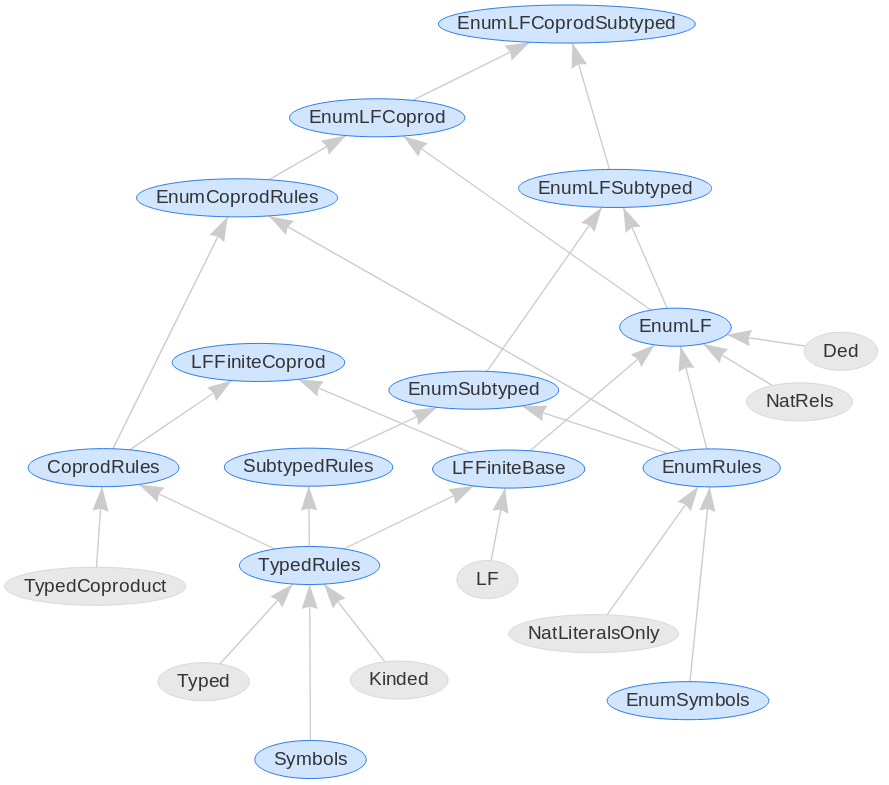
\includegraphics[width=0.7\textwidth]{img/lf-finite}
  \caption{A Modular Development Graph for Finite Types}\label{fig:lf:lfx:finite:devel}
\end{figure}
